Data augmentation techniques artificially generate different versions of a real dataset in order to increase its size. Machine learning models can benefit from data augmentation algorithms. A deep learning model with image augmentation outperforms a deep learning model without augmentation in terms of training loss (the penalty for a bad prediction), accuracy, validation loss, and accuracy.

 \begin{figure}[h]
	\centering
	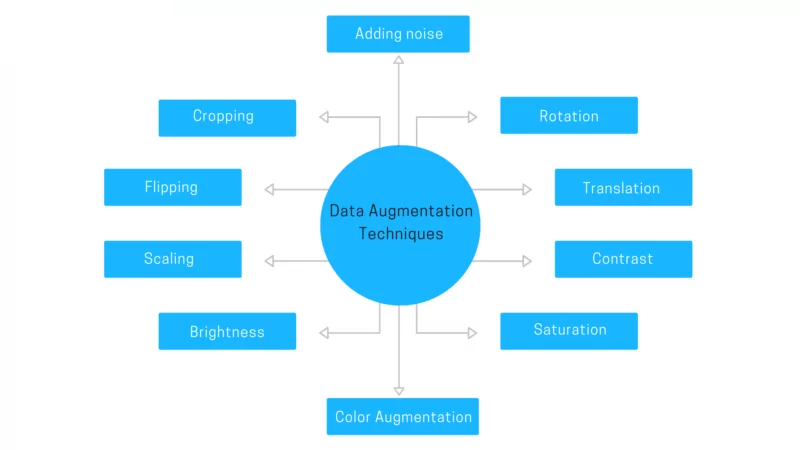
\includegraphics[width=0.8\textwidth]{figures/background/DataAugmentation.png}
	\captionsetup{labelformat=empty}
	\caption{\href{https://research.aimultiple.com/wp-content/webp-express/webp-images/uploads/2021/04/data-augmentation-techniques-800x450.png.webp}
	{Data Augmentation Techniques}}
\end{figure}

In the above figure we show the most common data augmentation techniques. All of the techniques purpose is to increase the current dataset size. We will use some of these techniques to increase our Dataset, but the main goal would be to create a GANs that will create new examples of the training set that we will use, which is consider an advanced method of data augmentation. In general, data augmentation would generate more training samples by introducing some modification to the original training data whilst keeping the
same semantic labels. Often it is considered as a regularization which can mitigate the notorious over-fitting problem. Data augmentation operations are often randomly applied to a training sample during training. The common augmentation operations include flipping, rotating, scaling, occluding, and color jittering and some other as it is shown in the figure above. \\

However, there are some limitations to this method. The main issue is that augmented data contain biases if the real dataset contains the same, and that confuses the model during the training. Moreover, data augmentation techniques like GANs are quite challenging since GANs generations also have some limitations, (some noticeable differences from the real data).